\def\QRCODE{TB_IPR_EXAM.2018_up2_pratique_matlabqrcode.png}
\def\QRPAGE{http://www.iptutorials.science/tree/master/TB_IPR/EXAM.2018/up2_pratique_matlab}
\mcorrectionsection{Matlab correction}

\subsection{Counting the number of ones in an array (5 pts)}
This function makes use of \minline{circshift} to generate the different configurations of the array.
\begin{matlab}
function n = countContiguousOnes(x)

nmax=0;

for i=1:length(x)
    x2 = circshift(x, i);
    f = find(diff([0,x2,0]==1));
    p = f(1:2:end-1);  % Start indices
    y = f(2:2:end)-p;  % Consecutive ones counts
    if (isempty(y))
        n=0;
    else
        n =max(y);
    end
    
    if n>nmax
        nmax=n;
    end
    
end

n = nmax;
end
\end{matlab}

\subsection{Access to elements in the Bresenham circle (5 pts)}
For a window \minline{w} of size \minline{2*W+1} by \minline{2*W+1}, we transforme the 2D indices of the Bresenham circle into 1D indices, in order to access to all the values in the circle.
\begin{matlab}
w= I(i-W:i+W, j-W:j+W);

indices_x = [4, 5, 6, 7, 7, 7, 6, 5, 4, 3, 2, 1, 1, 1, 2, 3];
indices_y = [1, 1, 2, 3, 4, 5, 6, 7, 7, 7, 6, 5, 4, 3, 2, 1];

M = 2*W+1;
idx = M * (indices_x - 1) + indices_y;

x = w(idx);
\end{matlab}

This finally give the following function that tests is a point is a FAST corner:
\begin{matlab}
function [res, n1, n2] = isFastCorner(I, i, j, W, t, nt)
% verifies if a point of coordinates (i,j) in image I is a FAST corner
% W is the window radius
% t is the threshold value
% nt is the minimum number of pixel to considere a corner, usually 12

w= I(i-W:i+W, j-W:j+W);
C1 = w > I(i,j)+t;
C2 = w < I(i,j)-t;

indices_x = [4, 5, 6, 7, 7, 7, 6, 5, 4, 3, 2, 1, 1, 1, 2, 3];
indices_y = [1, 1, 2, 3, 4, 5, 6, 7, 7, 7, 6, 5, 4, 3, 2, 1];

M = 2*W+1;
idx = M * (indices_x - 1) + indices_y;

n1 = countContiguousOnes(C1(idx));
n2 = countContiguousOnes(C2(idx));

if ((n1>=nt) || (n2>=nt))
    res = 1;
else
    res = 0;
end
end

\end{matlab}

\subsection{FAST corner detector (10 pts)}
Finally, the FAST corner detector consists in looping over all pixels and testing if the number of contiguous ones is higher than a threshold (in this case, we used 11).
\begin{matlab}
I = imread('square.png'); I = I(:,:,2);
%I = imread('sweden_road.png');
I = 255*uint8(I > 200);
tic
W=3;
t = 10;
C=uint8(zeros(size(I)));
N=uint8(zeros(size(I)));
for i=1+W:size(I, 1)-W
    parfor j=1+W:size(I,2)-W
        [res, n1, n2] = isFastCorner(I, i, j, W, t, 11);
        C(i, j) = res;
        N(i, j) = max(n1, n2);
    end
end

imshow(C, [])
\end{matlab}

The next code is used to save the image as a color image (see result in Fig.\ref{fig:exams:ipr:2019:results}). The structuring element size gives the size of the point (it is to be adapted to the size of the original image).

\begin{matlab}
I2 = repmat(I, 1, 1, 3);

SE = strel('disk', 15);
P = imdilate(255*C, SE);
I2(:,:,1) = max(I2(:,:,1), P);
I2(:,:,2) = min(I2(:,:,2), 255-P);
I2(:,:,3) = min(I2(:,:,3), 255-P);
imshow(I2, [])
toc

figure, imshow(N>=10, []);
\end{matlab}


\begin{figure}[htbp]
 \centering \subfloat[Result on the square.]{
\includegraphics[width=.3\linewidth]{square_result.png}}\hfill
 \subfloat[Result on the wild roar.]{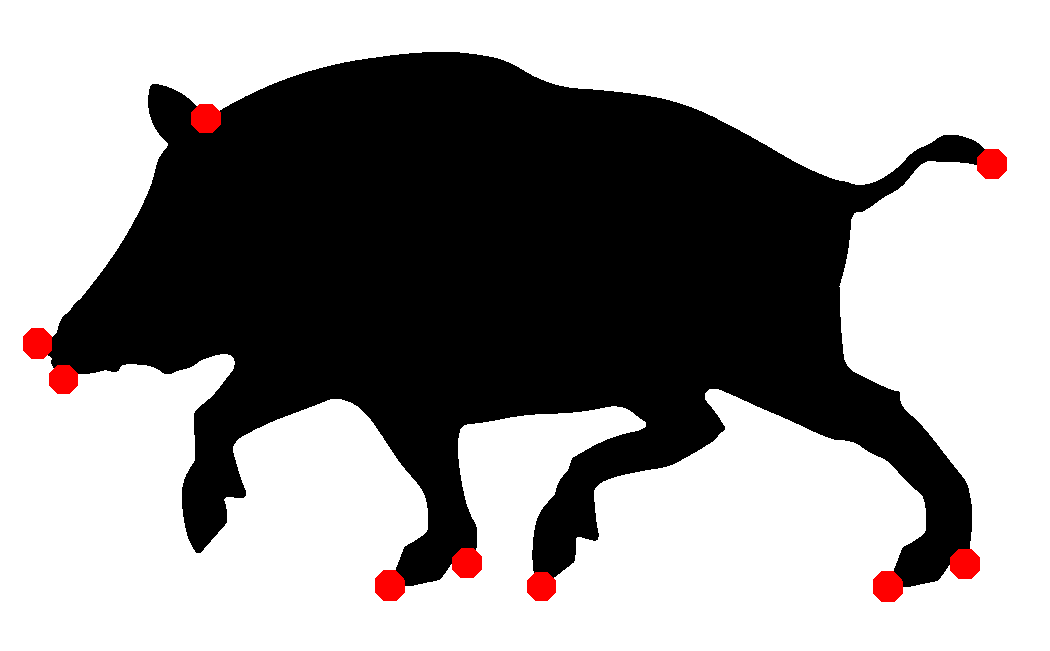
\includegraphics[width=.45\linewidth]{res_fast.png}}
 
 \caption{Expected results}
 \label{fig:exams:ipr:2019:results}
\end{figure}

